\documentclass{article}
\usepackage[utf8]{inputenc}
\usepackage[english]{babel}
\usepackage{amsthm}
\usepackage{amssymb}
\usepackage{mathcomp}
\usepackage{amsmath}
\usepackage{natbib}
\usepackage{array}
\usepackage{wrapfig}
\usepackage{multirow}
\usepackage{tabularx}
\usepackage{multirow}
\usepackage{graphicx}
\usepackage{geometry}
\usepackage{multicol}
\usepackage{blindtext}
\setlength{\columnsep}{1cm}
\usepackage[rightcaption]{sidecap}
\linespread{1.6}

\begin{document}

\begin{titlepage}
    \newgeometry{left=0.1cm,bottom=0.1cm,top=0.1cm,right=0.1cm}
    \centering
    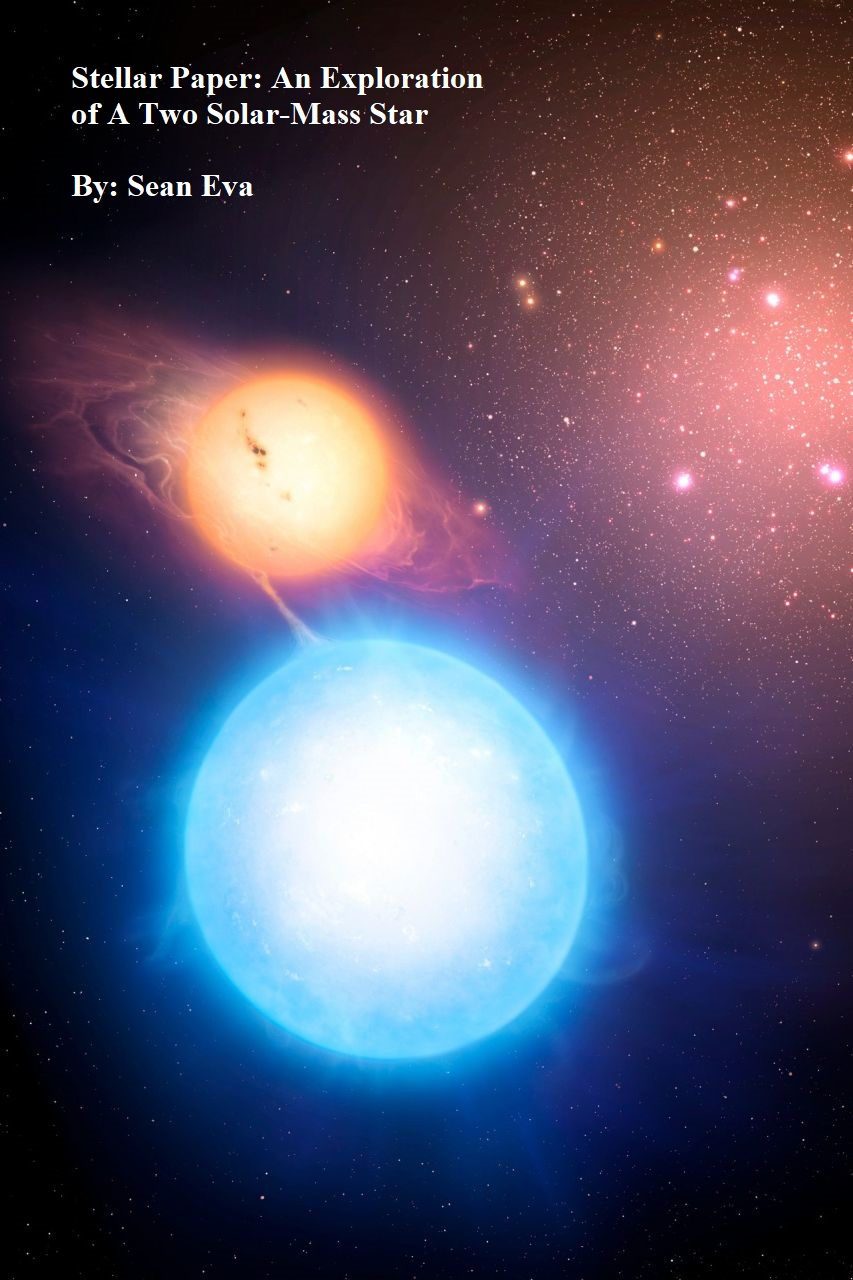
\includegraphics[width=18.485cm]{Cover.jpg}
    \restoregeometry
\end{titlepage}

\newgeometry{left=2.54cm,bottom=2.54cm,top=2.54cm,right=2.54cm}

Many people ask what we are made of. And it is simple to say the various compounds and the atoms that make up those compounds. But there is a lot more to those atoms that make up us and all the things that we use. Those atoms took thousands of years to be formed through the fusion reactions that take place in. These stars contain a lot of information about the formation of different elements. We are able to use different methods and formulas in order to analyze a star and learn its mysteries that allow us to understand a more foundational origin.\\

The purpose of this set of exercises is to create a comprehensive overview of a $2M_\odot$ star. Not only will this be a comprehensive overview of this star but it will also be a collection and evidence of my understanding of the course material and my ability to use and apply this information to a real world example with data to work with. I will use this data to analyze the star and compare it to a $1M_\odot$ star as well as another star of approximately $2M_\odot$.\\

\pagebreak

\begin{multicols}{2}

The first step in analyzing our $2M_\odot$ star is to compare it to some sort of standard. This standard will be a $1M_\odot$ star. We are going to compare the surface conditions of our $2M_\odot$ star to this $1M_\odot$ star. We will start with the more obvious. Our $2M_\odot$ star is twice as massive as a $1M_\odot$ star. The radius of our $2M_\odot$ is $1.258R_\odot$ or it is $1.58$ times the radius of the sun. This radius is greater than the radius of a $1M_\odot$ star as a $1M_\odot$ star only has a radius of $1.021R_\odot$. It is important to note that the radius of the star does not have a linear relation with the mass because as the star becomes more massive its gravity and pressure equilibrium of the star are different causing the star to have a different radius and will result in different life spans and outcomes. The total luminosity of our $2M_\odot$ star is about $22.612L_\odot$ or $22.612$ times the luminosity of the sun while the $1M_\odot$ star is approximately $0.861L_\odot$. The temperature of the $2M_\odot$ star on the surface is about $11218K$ whereas the $1M_\odot$ is about $5500K$. Next we are going to begin analyzing the internals of the $2M_\odot$ star. Using the given data, we are going to be taking a look at the temperature, density, luminosity, and mass with respects to a normalized radius of the star. This normalized radius is where we use the radius of the star in terms of the radius of the sun. First we will look at the mass of the star. As we begin from the center of the star and move outwards the \% mass that is accounted increases. However, the mass isn't accounted for linearly as we move outwards from the center of the star. It has a logarithmic pattern where the biggest increase is between $0.2$ and $0.6$ solar radii. This can be seen by referring to Figure \ref{fig:mass} where the mass \% is measured according to the normalized radius.\\

\end{multicols}

\begin{figure}
  \centering
  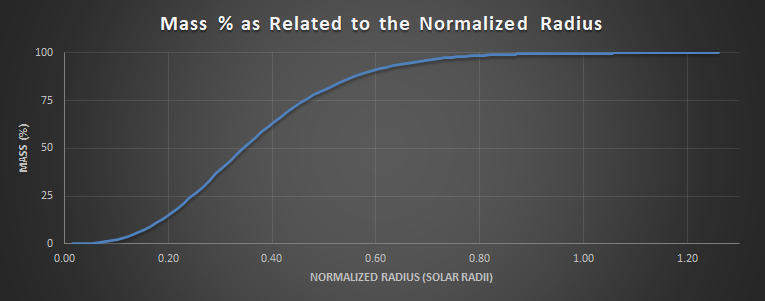
\includegraphics[width=0.9\textwidth]{mass.png}
  \caption{A graph showing the relationship of mass \% against the normalized radius.}
  \label{fig:mass}
\end{figure}

\begin{multicols}{2}

Next we will take a look the relationship between the normalized radius and the luminosity of our $2M_\odot$ star. If we take a look at the graph comparing the two values in Figure \ref{fig:lumino}. The relationship is very similar to the relationship between the mass and the normalized radius. The luminosity and normalized radius have a positive logarithmic relationship. The biggest part of the luminosity change is between $0.1$ and $0.2$ solar radii for the star. We can further analyze this luminosity and normalized radius relationship and determine that approximately $99\%$ of the luminosity is produced within $0.342$ solar radii from the center of the star. This region we will define as the core of the star, and we will come back to this region after analyzing the rest of these relationships. We can see the relationship between the luminosity \% change and the normalized radius of the star in Figure \ref{fig:lumin}.\\\\\\\\\\
\end{multicols}

\begin{figure}
  \centering
  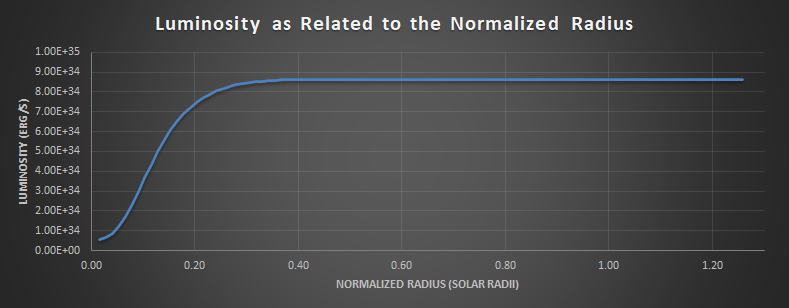
\includegraphics[width=0.9\textwidth]{lumino.png}
  \caption{A graph showing the relationship of luminosity against the normalized radius.}
  \label{fig:lumino}
\end{figure}
\begin{figure}
  \centering
  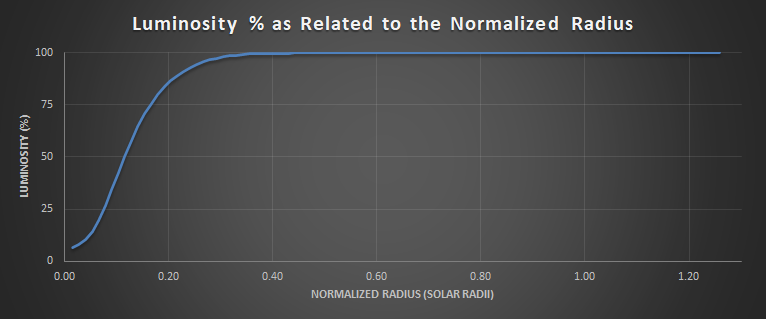
\includegraphics[width=0.9\textwidth]{lumin.png}
  \caption{A graph showing the relationship of luminosity \% against the normalized radius.}
  \label{fig:lumin}
\end{figure}

\begin{multicols}{2}

Now we are going to discuss something that has a slightly different relationship with the normalized radius of the star. The temperature of our $2M_\odot$ star has a negative logarithmic relationship with the normalized radius. This decrease is much more gradual than that of the mass \% and the luminosity \%. The majority of the decrease of the temperature is between $0.1$ and $0.6$ solar radii. These relationships can be seen in Figure \ref{fig:temp}. 

\end{multicols}

\begin{figure}
  \centering
  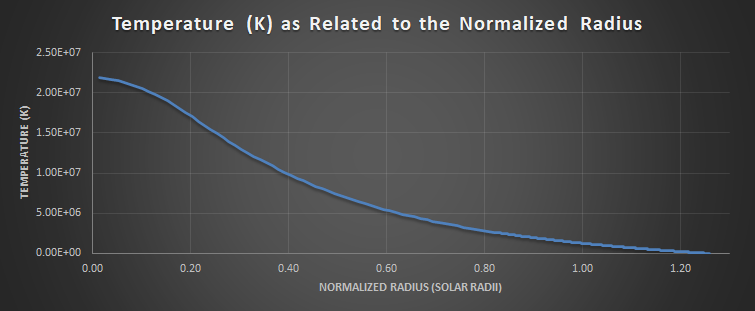
\includegraphics[width=0.9\textwidth]{temp.png}
  \caption{A graph showing the relationship of temperature ($K$) against the normalized radius.}
  \label{fig:temp}
\end{figure}

\begin{multicols}{2}

Having seen the relationship of the temperature and luminosity of the $2M_\odot$ star with respect to the normalized radius, we are now able to relate these three values together using the Stefan-Boltzmann law. The formula is that $L=4\pi R^2\sigma T^4$. We would then be able to compare these values to that of the $1M_\odot$ to find a ratio of the luminosities between the stars. Finally, the last relation we will analyze is between the density of the star and the normalized radius. The density and normalized radius relationship is similar to the relationship between temperature and the normalized radius in that it has a negative logarithmic relationship. The greatest decrease in density of the star is between $0.1$ and $0.4$ solar radii. This can be seen by referring to Figure \ref{fig:dense}. This internal density is caused as a result of the results to the PP1 reaction where hydrogen gets turned into helium. This helium is more dense than the hydrogen and therefore sinks down into the core of the star and then around the core forms a shell of hydrogen. Eventually too the helium begins to fuse after the helium flash where it then forms carbon and forms a carbon core with a helium shell followed by a hydrogen shell. So the gradient between the core and the subsequent shells is where this change in density comes from.

\end{multicols}

\begin{figure}
  \centering
  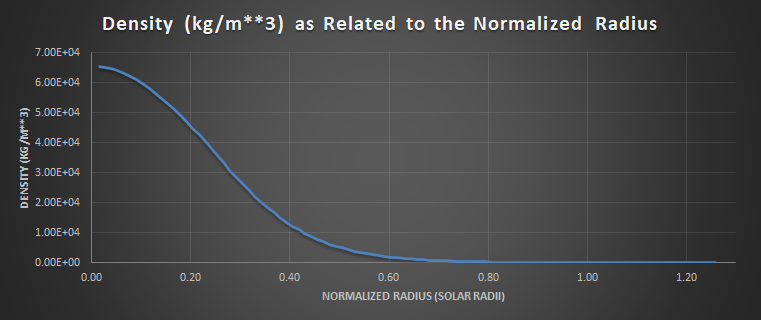
\includegraphics[width=0.9\textwidth]{dense.png}
  \caption{A graph showing the relationship of density ($kg/m^3$) against the normalized radius.}
  \label{fig:dense}
\end{figure}

\begin{multicols}{2}

Now we will return to the region we defined as the core. Again this region is where approximately $99\%$ of the luminosity of the star is produced. For our $2M_\odot$ that occurs withing approximately $0.342$ solar radii from the center of the star. This core region is both radiative and convective. The inner region of the core is where the convective energy transfer takes place and the particles are physically moving around transferring the energy whereas the outer region of the core the energy is transferred radiatively. The volume of the whole star can be determined using the volume of a sphere formula: $V = \frac{4}{3}\pi r^3$ and we can use the radius in terms of the solar radii. The volume of the core is $V = \frac{4}{3}\pi (0.342)^3 = 0.168$ cubic solar radii. We can then compare this to the total volume of the star, which is $V = \frac{4}{3} \pi (1.258)^3 = 8.339$ cubic solar radii. This means that the core region comprises approximately $\frac{0.168}{8.339}*100 = 0.020*100 = 2.0\%$ of the total star. 

\end{multicols}

\begin{figure}
  \centering
  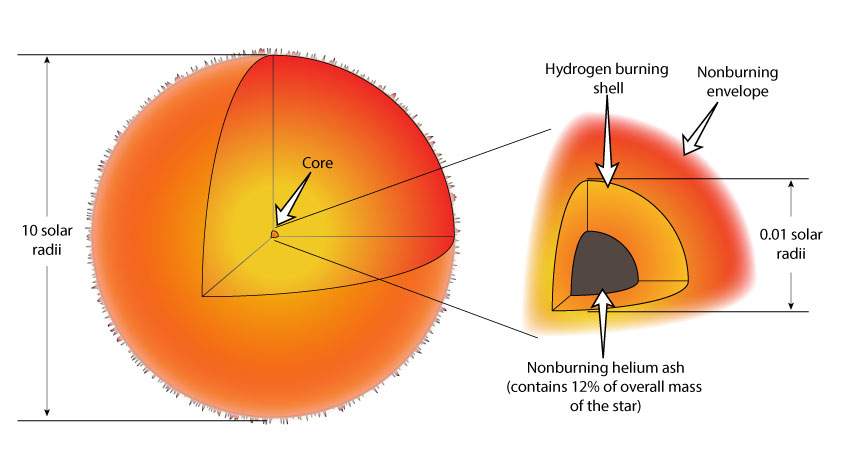
\includegraphics[width=0.9\textwidth]{Core.jpg}
  \caption{This is an illustration of the core of a 10 solar radii star that shows the relative size of the core in comparison to the rest of the star. Additionally, there is the helium core that is surrounded by the shell of helium that is still fusing to create more helium over time. (Emma 2021)}
  \label{fig:core}
\end{figure}

\begin{multicols}{2}

We can now further investigate the properties of our core region. We will calculate the mass of the core. We can refer back the data used for Figure \ref{fig:mass} to see the core region contains approximately $49.5\%$ of the total mass of the star. That is to say that the core is approximately $0.495*2 = 0.99M_\odot$ which is approximately $0.99*1.989*10^30 = 1.969*10^{30}\text{ kg}$. Using the central core temperature, density, and composition we are going to calculate the amount of energy released per gram per second of the proton-proton (PP) reaction using the formula: $\epsilon_{pp} = C_{pp}\rho X^2 (\frac{10^6}{T})^\frac{2}{3}e^{-33.8(\frac{10^6}{T})^\frac{1}{3}}$ where $C_{pp} = 2.5*10^6$. Then we can use our central core temperature of $2.19*10^7K$, density of $6.57*10^1 g/cm^3$, and the composition is $X=0.7, Y=0.292, Z=0.008$. This results in $\epsilon_{pp} = (2.5*10^6)(6.57*10^1)(0.7)^2(\frac{10^6}{2.19*10^7})^{\frac{2}{3}}e^{-33.8(\frac{10^6}{2.19*10^7})^{\frac{1}{3}}} = 58.26\text{ ergs}$. Similarly we can use $\epsilon_{CNO} = C_{CNO}\rho XX_{CNO}(\frac{10^6}{T})^{\frac{2}{3}}e^{-152.3(\frac{10^6}{T})^{\frac{1}{3}}}$ where $C_{CNO} = 9.5*10^{28}$ and $X_{CNO} = \frac{1}{3}Z = \frac{1}{3}*0.008 = 0.0027$. Then this implies that $\epsilon_{CNO} = (9.5*10^{28})(6.57*10^1)(0.7)(0.0027)(\frac{10^6}{2.19*10^7})^\frac{2}{3}e^{-152.3(\frac{10^6}{2.19*10^7})^{\frac{1}{3}}} = 3442.88\text{ ergs}$. We can then see the relationship between energy productions of the CNO cycle and the PP chain at various temperatures in Figure \ref{fig:energyrate}.

\end{multicols}

\begin{figure}
  \centering
  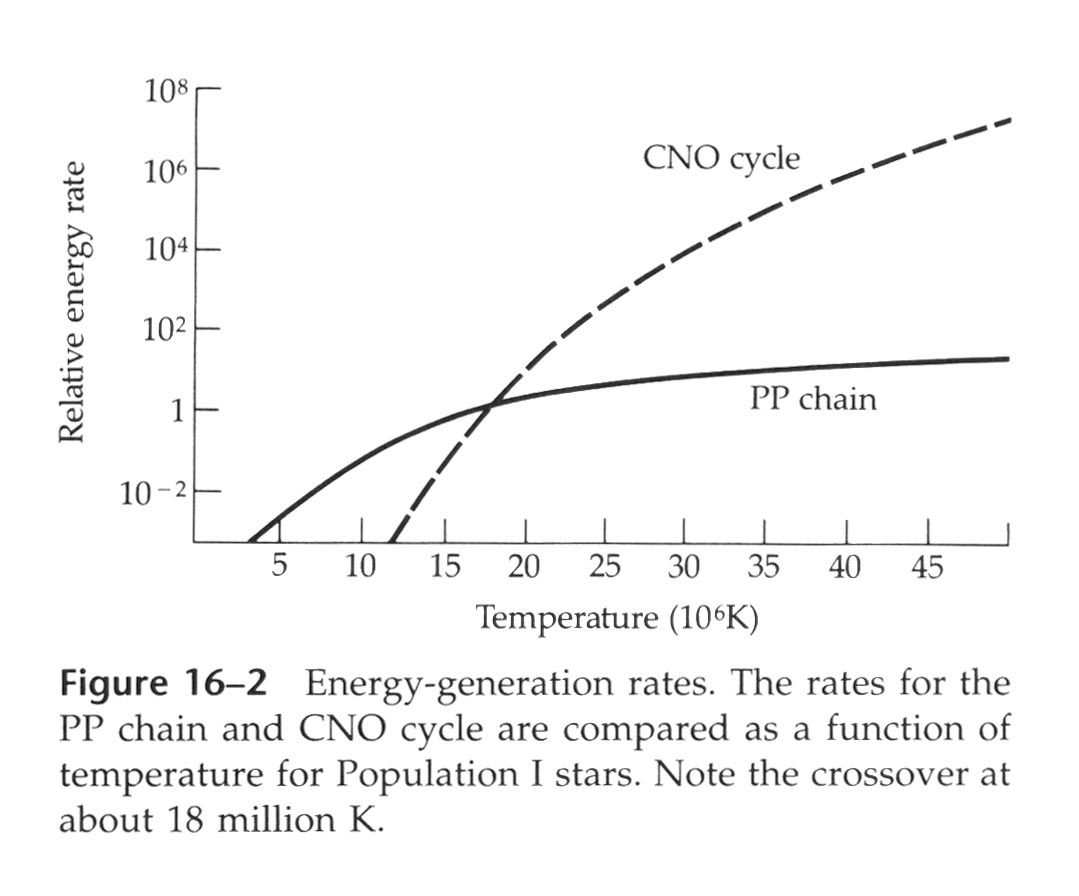
\includegraphics[width=0.46\textwidth]{Energy_Rates.jpg}
  \caption{A graph showing the relationship between the energy generation rates of the CNO cycle and the PP chain at different temperatures. (Zeilik \& Gregory, 1998)}
  \label{fig:energyrate}
\end{figure}

\begin{multicols}{2}

We can then calculate the ratio of the energy released between the PP chain the the CNO cycle as $\frac{58.26}{3442.88} = 0.0169$. This ratio implies that a PP chain is only producing about $1.69\%$ the amount of energy a CNO cycle is producing per gram per second. Now what if we assumed that $100\%$ of the surface luminosity of the $2M_\odot$ star is generated by the Proton-Proton I (PPI) chain. Then it would be interesting to know the amount of reactions required in order for the luminosity to be made up out of the PPI chain. The amount of energy released from a single PPI chain is approximately $26.729 \text{ MeV} = \frac{26.729}{6.242*10^{12}} = 4.282*10^{-12}$. And the luminosity of the star in joules is approximately $22.612(3.846*10^{26}) = 8.697*10^{27}\text{ J}$. This implies that the amount of reactions needed in order to produce this luminosity is approximately $\frac{8.697*10^{27}}{4.282*10^{-12}} = 2.031*10^{39}$ reactions per second. 

\end{multicols}

\begin{figure}
  \centering
  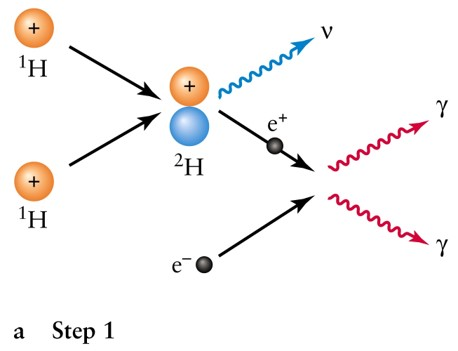
\includegraphics[width=0.45\textwidth]{PP1.jpg}
  \caption{This is an illustration of what happens during the PP1 chain reaction. This is the first step of the reaction where two hydrogen-1 atoms collide together to produce a hydrogen-2 atom and a positron and a neutrino. (\textit{Universe})}
  \label{fig:PP1}
\end{figure}
\begin{figure}
  \centering
  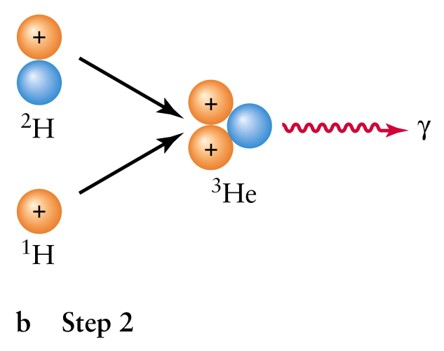
\includegraphics[width=0.45\textwidth]{PP2.jpg}
  \caption{This is an illustration of what happens during the PP1 chain reaction. This is the second step of the reaction where a hydrogen-1 and a hydrogen-2 atoms collide together to produce a helium-3 and a gamma ray.\textit{Universe}}
  \label{fig:PP2}
\end{figure}
\begin{figure}
  \centering
  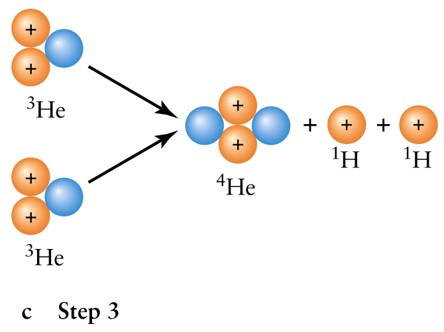
\includegraphics[width=0.45\textwidth]{PP3.jpg}
  \caption{This is an illustration of what happens during the PP1 chain reaction. This is the third and final step of the reaction where two helium-3 atoms combine to form a helium-4, the desired result, and two helium-1 atoms with no erroneous byproducts.\textit{Universe}}
  \label{fig:PP3}
\end{figure}

\begin{multicols}{2}

In order for the complete PPI chain reaction to occur, the chain requires a total of 6 hydrogen-1 atoms. This means that in order for there to be $2.031*10^{39}$ that means that we need $6*(2.031*10^{39}) = 1.219*10^{40}$ atoms of hydrogen to be processed per second. This converts to approximately $(1.219*10^{40})(1.67*10^{-27}) = 2.036*10^{13}$ kgs of hydrogen. However, since the final step of the PPI chain has a byproduct of 2 hydrogen-1 atoms, as can be seen in Figure \ref{fig:PP3}. This means that $\frac{2}{3}(2.036*10^{13}) = 1.357*10^{13}$ kgs of hydrogen that get converted into energy per second. Additionally from the luminosity of the $2M_\odot$ star we can use it to find the absolute magnitude of the star by comparing it to the absolute magnitude of the $1M_\odot$ star. We are given that the absolute magnitude of the $1M_\odot$ star is 4.75 mag. We can use the formula: $\Delta m = m_1-m_2 = 2.5\log(\frac{F_2}{F_1})$ where we will say star 1 is the $2M_\odot$ star and that star 2 is the $1M_\odot$ star and the luminosity of the the $1M_\odot$ star is approximately $0.86071$ Lsun. This means that the absolute magnitude of the $2M_\odot$ star is approximately $m_1 = 2.5\log(\frac{0.86071}{22.612})+4.75 = 1.201$ mag. Having a lower absolute magnitude means that the $2M_\odot$ star is actually more luminous than the $1M_\odot$ star which is obvious from the data values alone, but this is more a representation on another scale of the comparison between these two stars. Now using the temperature of the $2M_\odot$ we are going to determine the spectral type of the star. We will be referring to the Hertzsprung-Russell Diagram (HR Diagram) from \textit{Universe} by Freedman. Geller, and Kaufmann in Figure \ref{fig:hrd1}

\end{multicols}

\begin{figure}
  \centering
  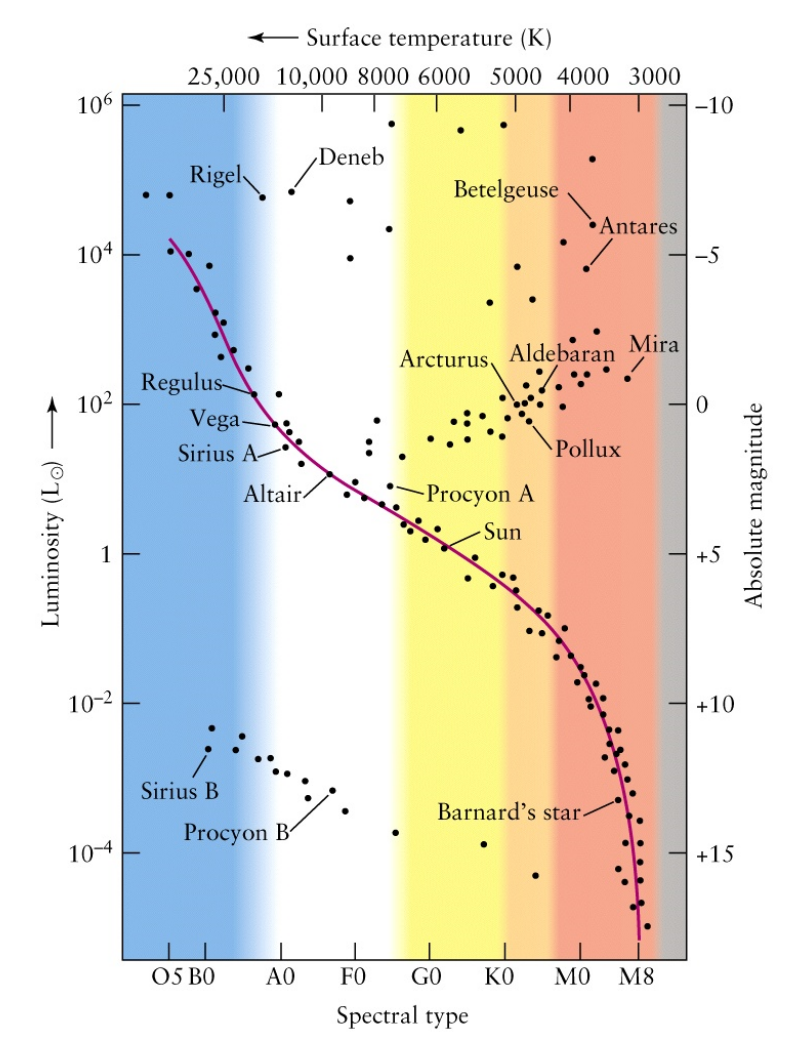
\includegraphics[width=0.3\textwidth]{HRD1.png}
  \caption{This is an HR Diagram that we can use to compare the surface temperature, luminosity, absolute magnitude, and spectral type of stars.}
  \label{fig:hrd1}
\end{figure}

\begin{multicols}{2}

Given that the surface temperature of the $2M_\odot$ star is $11218.4K$ that means that the star is around an A3 spectral type star. Since the classification of the star is in the A category, that means that the star's spectral graph has the strongest hydrogen lines. Therefore on an absorption spectrum, like we see in Figure \ref{fig:spectraltypes1} with A0 and A5 stars, there will be black lines where the hydrogen series of wavelengths would be located, and in an emission spectrum of light, there would be colored lines where the hydrogen series of wavelengths would be located.

\end{multicols}

\begin{figure}
  \centering
  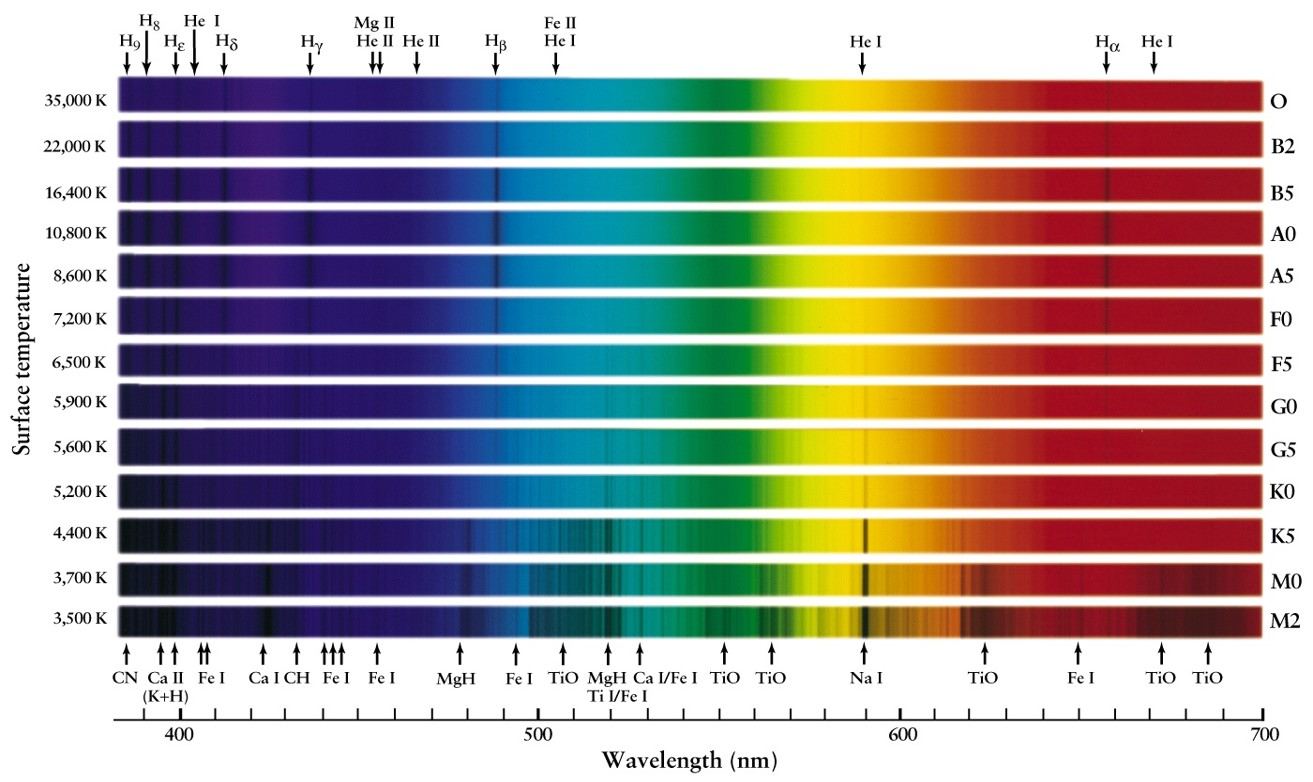
\includegraphics[width=0.86\textwidth]{Spectral_Types1.jpg}
  \caption{This is a set of absorption spectra. We are focused on the examples of A0 and A5 as our star is around an A3 star. We notice that the hydrogen series lines are darkened as there is no rays to absorb for these wavelengths.\textit{Universe}}
  \label{fig:spectraltypes1}
\end{figure}

\begin{multicols}{2}

Instead of using only the temperature to determine the spectral type of the star, we could use the mass of the star. We can use another HR Diagram from \textit{Universe} that is based on the mass of the stars along the main sequence of stars. We will us Figure \ref{fig:HRD2}. This figure tells us that for a $2M_\odot$ star should have a temperature of around $9000K$. Then if we refer back to Figure \ref{fig:hrd1} we would find that the star is now an A5 star. This star has roughly the same hydrogen line strength order but is slightly cooler in temperature.

\end{multicols}

\begin{figure}
  \centering
  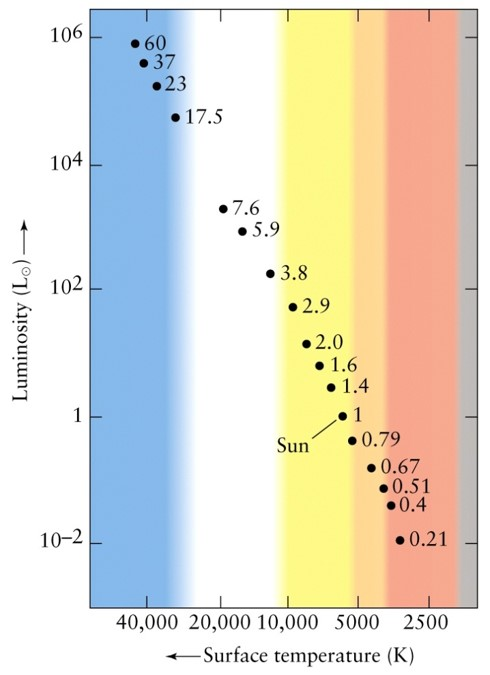
\includegraphics[width=0.43\textwidth]{HRD2.jpg}
  \caption{This is an HR Diagram that is based on the masses of the stars along the main sequence. We are able to use this HR diagram to get the temperature associated with a $2M_\odot$ star that we can use with our other HR Diagram.\textit{Universe}}
  \label{fig:HRD2}
\end{figure}

\begin{multicols}{2}

In these HR Diagrams there is an important band of stars known as the main sequence. The main sequence is a continuous band of stars. The sun lies along the main sequence and is where stars will spend most of their lifetime. Our sun for example is estimated to live on the main sequence for about $10*10^9$ years. In order to estimate how long the $2M_\odot$ star will live on the main sequence, we can use the formula $\tau = \frac{10*10^9}{M^3}$. Therefore, the $2M_\odot$ star will live on the main sequence for approximately, $\tau = \frac{10*10^9}{2^3} = 1.25*10^9$ years. Which is $\frac{1}{8}$th the amount of time the sun will live on the main sequence. 
Now that we've done an extensive analysis of our model $2M_\odot$ star, we can now work to compare it to a somewhat similar mass star Fomalhaut. The mass of Fomalhaut is just a little less than that of $2M_\odot$. The radius of Fomalhaut is much greater than the model as it is $1.842R_\odot$ which is $0.584 R_\odot$ larger than the model $2M_\odot$ star. The luminosity of Fomalhaut is less than that of the model only having a luminosity of $16.63L_\odot$. Lastly, the temperature of Fomalhaut is less than that of the model $2M_\odot$ star, Fomalhaut has a temperature of about $8590K$ while the model is about $11218K$ on the surface. Fomalhaut also has a greater absolute magnitude than our model did. The absolute magnitude of Fomalhaut is 1.72 mags while the model had an absolute magnitude of about 1.201 mags. This implies that the luminosity of Fomalhaut is less than that of the model which is true. 

\end{multicols}

\begin{figure}
  \centering
  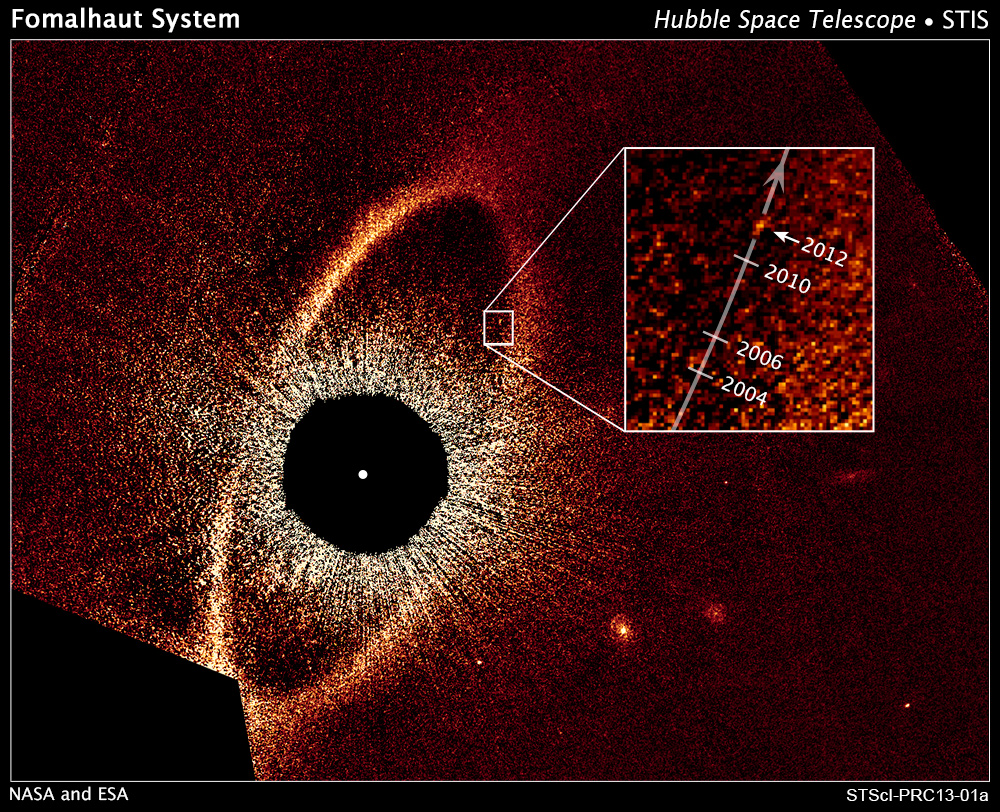
\includegraphics[width=0.86\textwidth]{Fomalhaut.jpg}
  \caption{This is an image of the Fomalhaut System where the central dot of the event is the star Fomalhaut. This is an image from NASA discussing planetary orbit around Fomalhaut.(Harrington \& Villard, 2013)}
  \label{fig:fomalhaut}
\end{figure}

\pagebreak

From this exploration we were able to make a sensible comparison between a model $2M_\odot$ star with a $1M_\odot$ star. Not only were we able to make a comparison between two model stars, we are able to make a deep analysis of the model where we are able to uncover most of the major pieces of information about the star that we could then ultimately use to compare it to an actual star of similar mass, which was Fomalhaut. We were able to see, while the model wasn't a perfect representation of Fomalhaut, it is still an amazing example to demonstrate the knowledge from the course and applying it to the real world where all the processes that we used to analyze this star would still apply to a normal star given the proper information. 


\pagebreak

References\\
Emma. \textit{What Happens in an Expanding Star's Core?}. URL: https://scienceatyourdoorstep.com/2020/04/06/what-happens-in-an-expanding-stars-core/. (accessed: 25.11.2021)\\\\
Introductory Astronomy and Astrophysics, 4th ed, Zeilik \& Gregory, Thomson Learning, 1998\\\\
J.D. Harrington Ray Villard. \textit{NASA's Hubble Reveals Rogue Planetary Orbit for Fomalhaut B}. URL: https://www.nasa.gov/mission$\_$pages/hubble/science/rogue-fomalhaut.html. (accessed 25.11.2021)\\\\
Sowell et al, Astronomical Journal, 134, 1089, 2007\\\\
\textit{Universe}, Kaufmann, W.H.Freeman and Company.

\pagebreak

\end{document}
